\documentclass[a4paper]{article}
\usepackage[utf8]{inputenc}
\usepackage[english]{babel}
\usepackage{microtype,etex,listings,color,parskip, graphicx, float}
\usepackage[margin=2cm]{geometry}
\usepackage[hidelinks]{hyperref}
\usepackage[htt]{hyphenat}


\newcommand{\secref}[3][green]{\href{#2}{\color{#1}{#3}}}%
\newcommand{\urlref}[3][blue]{\href{#2}{\color{#1}{#3}}}%

\usepackage{wasysym}

\lstset{
    language=C,
    tabsize=2,
    showstringspaces=false,
    breaklines=true,
    basicstyle=\ttfamily,
    keywordstyle=\color[rgb]{0.1,0.3,0.7}\ttfamily,
    stringstyle=\color[rgb]{0.7,0.1,0.3}\ttfamily,
    commentstyle=\color[rgb]{0.3,0.4,0.3}\ttfamily,
    columns=fixed,
    numberstyle=\sffamily\scriptsize,
    backgroundcolor=\color[rgb]{0.95,0.95,0.95},
    frame=lines,
    framexleftmargin=5pt,
    numbers = left,
    numberstyle = \footnotesize,
}



\lstdefinelanguage{JS}{
    keywords={ var, typeof, new, true, false, catch,
        function, return, null, catch, switch, let, var, if, of, in,
    for, while, do, else, case, break, const},
    keywordstyle=\color{blue}\bfseries,
    ndkeywords={class, export, boolean, throw, implements, import, this},
    ndkeywordstyle=\color{darkgray}\bfseries,
    identifierstyle=\color{black},
    sensitive=false,
    comment=[l]{//},
    morecomment=[s]{/*}{*/},
    commentstyle=\color[rgb]{0.3,0.4,0.3}\ttfamily,
    stringstyle=\color{red}\ttfamily,
    morestring=[b]',
    morestring=[b]"
}

\lstset{
    language=JS,
    extendedchars=true,
    basicstyle=\footnotesize\ttfamily,
    showstringspaces=false,
    showspaces=false,
    numbers=left,
    columns=flexible,
    numberstyle=\tiny,
    numbersep=9pt,
    tabsize=2,
    breaklines=true,
    showtabs=false,
    captionpos=b,
}

\lstdefinelanguage{DPL}{
    keywords={ fn, print, int, float, bool, var, typeof, new, true, false, catch,
        function, return, null, catch, switch, let, var, if, of, in,
    for, while, do, else, case, break, const},
    keywordstyle=\color{blue}\bfseries,
    ndkeywords={class, export, boolean, throw, implements, import, this},
    ndkeywordstyle=\color{darkgray}\bfseries,
    identifierstyle=\color{black},
    sensitive=false,
    comment=[l]{//},
    morecomment=[s]{/*}{*/},
    commentstyle=\color[rgb]{0.3,0.4,0.3}\ttfamily,
    stringstyle=\color{red}\ttfamily,
    morestring=[b]',
    morestring=[b]"
}

\lstset{
    language=DPL,
    extendedchars=true,
    basicstyle=\footnotesize\ttfamily,
    showstringspaces=false,
    showspaces=false,
    numbers=left,
    columns=flexible,
    numberstyle=\tiny,
    numbersep=9pt,
    tabsize=2,
    breaklines=true,
    showtabs=false,
    captionpos=b,
}

\begin{document}
\tableofcontents


\title{DPCC: DParo's Own C-Alike Compiler}
\author{Davide Paro}
\date{December 2020}

\maketitle

\section{Assignment Description}
This project is about an assignment for a course on \textbf{Compilers}
at the department of Computer Engineering Master Degree Padova (ITA).


The assignment consists in implementing a toy compiler for a toy language. More emphasis
is put on the implementation for the frontend side (input, lexing, parsing, type checking), while
the backend side is stubbed out by a simple 3AC \footnote{3AC: Three Address Code} Intermediate Code
generator.
We are free to design the syntax of this toy language however we like.

The assignment specs out the how the compiler should be composed.
We can in fact distinguish these macro components:

\begin{itemize}
\item \textbf{Input Stage} deals with the input byte stream that composes
    the source of the program.
\item \textbf{Lexer/Scanner} has the purpose of grouping characters (lexical analysis)
    together to compose compunded
    structures (called tokens). For the project assignment we can use \textbf{Flex} to aid in
    the implementation of the scanner.
\item \textbf{Parser} for performing the syntax analysis. It is what defines the look \& fell
    (grammar) of the language. For the project assignment we can use \textbf{Bison} to aid in the
    implementation of an LR parser.
\item \textbf{Intermediate Code Generator}. The ultimate purpose of a compiler is to produce something
    useful. In this project assignment we are not asked to implement a proper backend. Instead,
    we need to emit a 3AC representation of our input program. More in this later.
\end{itemize}

Three Adress Code (3AC) is a type of intermediate code generator which is both easy to understand and to emit.
In 3AC, each statement can only have 1 operand at the left hand side of the assignment, and at most 2 operands at the right hand side
of the assignment, and an operator driving the operation that should be performed.

You can view more about 3AC at the following \urlref{https://en.wikipedia.org/wiki/Three-address_code}{Wikipedia link}, or here \urlref{https://www.geeksforgeeks.org/three-address-code-compiler/}{Geeks4Geeks link}.

In practice, the emitted 3AC code is on itself a partially valid C program, it's only missing variable
declarations at the top for each temporary variable. Control flow is allowed to be implemented
trough the usage of C labels and simple if conditional followed by a goto statement. Inside
the if conditional there can only be a single element composing the expression.

The project assignment requires the following features that should be developed for the language:

\begin{itemize}
    \item Variables declaration, initialization and assignment
    \item Scoping. Variable names are reusable in different scopes. Variable
        shadowing may or may not warn/fail/pass depending on the design choices.
    \item Only 2 types of variables: integers, booleans
    \item Assignment statements, print statements, if statements, and at least 1 loop statement at our liking
    \item Handling of simple mathematical expressions that we can encounter in common programming
        languages: addition, subtraction, multiplication, division, modulo, etc \dots
    \item \textbf{Function definition, function calls, and custom user definable types are not required}
\end{itemize}

The unpatient reader can already jump tho the \hyperref[appendix_a]{Appendix A} to quickly look at an
example program of the designed language. \hyperref[appendix_a]{Appendix A} lists the program
source, the output which is generated by running said program and the 3AC that the compiler emits
when performing the compilation.

\clearpage

\section{DPL and dpcc: A quick peak at the language and at the compiler}

\textbf{DPL} and \textbf{DPCC} are respectively the \textbf{name of the language} and the
\textbf{name of the implemented compiler}. They are named after their author.

From now on \textbf{DPL} and \textbf{DPCC} will be used for brevity for refering to the language and to the compiler.
We will use \textbf{dpcc} (all lowercase) instead, to refer to the actual executable where the compiler lives.

That being said \textbf{DPCC} (all UPPERCASE) and \textbf{dpcc} (all lowercase) are mostly used interchangeably to refer to the same thing.


\subsection{DPL: Structure of the language}

\textbf{DPL} is mostly a C-alike compatible language, in fact it borrows most of its syntax and semantics.
\textbf{DPL} is also inspired by the following programming languag: \textbf{Rust} \&
\textbf{JS} especially in the syntax used to perform variable declarations (usage of the keyword \textbf{let}).

\textbf{Rust} is a modern system programming language with strong typing guarantees.
Among all the interesting features that Rust provides one of them is type deduction.
Thanks to Rust's strong typing guarantees and thanks to strong type deduction rules implemented
inside the \textbf{rustc} compiler, Rust
allows one to declare variables with a very low-weight syntax, similar
to a syntax provided from a typical dynamic language (for example JS).

\textbf{DPL}, like Rust, also have a very simple form of a type deduction system.
It is not even remotely close to the Rust type deduction system, but still it
allows the user of the language to not always need to specify the type of each variable in a declaration.
How this is achieved will be described in later sections.

In \textbf{DPL}:

\begin{itemize}
\item Spaces and newlines mostly do not matter, they simply introduce token boundaries.
\item Comments start with the double forward slash `\texttt{//}', and C-style multiline comments are
instead not supported (at the time of writing).
\end{itemize}



Here follows a chunk of \textbf{DPL} code to show off the syntax and some of the language features:

\begin{lstlisting}[language=DPL]
// Print statement with immediate C-style strings. C-style strings can only be used inside print statement
print("Hello world\n");

// Variable declaration and initialization
let a = 10;          // Integer Type deduced
let f = 10.0;        // Float type deduced
let b = false;       // Boolean type deduced

// Explicit types
let i: int = 0xffff & ~0xb00111;
let f: float = 10.0 + 20.0 ** 2;

// Immediate values can be printed
print(10);
print(30 + 4);

// Variables can be printed
print(i);       // Print integer
print(f);       // Print float

// Casting can be used to enforce type conversion
let myInt: int = int(10.00f);
let myFloat = float(0xFF);

// Type deduction
let b = (10 < 20);   // Boolean type is deduced
let f = 1 + 2.0f;    // Float type is deduced (the 1 is upcasted to a float)

// Scoping and restricting variable declarations to the current scope
{
    // Simple single dimension arrays declaration
    let buf_i: int[100];            // Known size integer array
    let buf_f: float[100];          // Known size float array

    // Integer array with deduced size from the RHS initializer list
    let buf = [ 10, 20, 30, 40, 50 ];
    let fs: float[] = [ 0.1, 0.2, 0.3, 0.4, 0.5 ];

    // Arrays can be printed
    print(buf);
}

let buf: int[100];

// Control flow
for (let i = 0; i < 100; i++) {
    buf[i] = i ** 2;

    if (buf[i] == 10) {
        print("buf[i] is 10!!!\n")
    }
    else if (buf[i] == 20) {
        print("buf[i] is 20!!!\n");
    }
    else {
        print("None of above\n");
    }
}
\end{lstlisting}

The cool thing about \textbf{DPL}, is that it is \textbf{almost a Javascript subset}.
That is one can simply copy the \textbf{DPL} code, strip the type information (if they're used
anywhere) by manual editing or automatically, and paste the same code into a browser console to evaluate as JS code.
With a couple modifications here and there (for example arrays with no initalizer list must be converted into a valid
JS array), one can
test if the compiler \textbf{dpcc} is producing the correct output by simply
evaluating the same code in a browser console.

This example shows how to convert \textbf{DPL} into \textbf{JS} by manual editing:

\begin{lstlisting}[language=DPL]
// This is a chunk of DPL code
let a = 10;                     // This is also valid JS code
let b = [ 10, 20, 30, 40 ];     // This is also valid JS code
let c: int = 10;                // Mostly valid JS code, remove the type info and the colon
let d: int[1024];               // Js arrays grow on demand automatically when touching elements.
                                // No need to specify neither type nor number of elements

print(d);                       // Valid JS code if function print were to be defined
\end{lstlisting}

Here's the equivalent JS code:

\begin{lstlisting}[language=JS]
// This is the equivalent Javascript
const print = console.log;      // Define it once at the top of the script

let a = 10;                     // Same as before
let b = [ 10, 20, 30, 40 ];     // Same as before
let c = 10;                     // Just strip the int type
let d = [];                     // Just initalizing with an empty array is enough

print(d);                       // Works because print is defined at the top
\end{lstlisting}

Most other \textbf{DPL} syntax and features, like code blocks, conditionals, loops \dots etc are valid JS code
thanks on how the grammar for \textbf{DPL} was defined.

For now \textbf{dpcc} supports only 5 types: \texttt{bool, int, float, string, bool[], int[], float[]}.
Only single dimensions array are for now supported. So arrays do not generalize to any number of dimensions.

Most of these types have full on semantics, meaning that the compiler can deduce
a type of an expression given the types of its operand. In some cases it can reject
the code if the operands of an expression have invalid types.
At the current time of writing, \texttt{string} types are quirky, meaning that
they don't have a full type tracking inside
the compiler like other types do.
The compiler still knows what a string is, and in it marks correctly \textbf{string literals} as
a \texttt{string} type, but strings undergo different semantics.
They cannot be assigned or operated on like a variable, but instead,
they can only be used as a parameter to the print statement.


\subsection{DPCC: Using the compiler}

The \textbf{dpcc} compiler is written in the \textbf{C} language. Unfortunately at the current time
of writing \textbf{dpcc} works only under Unix like operating systems. The compiler has
been tested under \textbf{Ubuntu 20.10}, Ubuntu 20.04, and macOS 10.15. The
compiler was developed by his author using an \textbf{Ubuntu 20.10} machine, while the other distro/OS
were tested thanks to \emph{Github Actions} automated build-check cycles. Windows builds
failed due to MSVC rejecting the source code of \textbf{dpcc} cause it contains some GCC
extensions and some hard coded unix syscalls.
In short words \textbf{dpcc} can be only compiled with either GCC or CLANG compilers
and executed in a Unix/Posix compatible operating system.

If you would like to build the compiler yourself from scratch please refer to the \urlref{https://github.com/dparo/dpcc/wiki}{Project WIKI}\footnote{\urlref{https://github.com/dparo/dpcc}{Github Repo Link}}

The compiler can and should be invoked from the commandline. The \textbf{dpcc} executable
is self contained and doesn't reach for any implicit external asset and thus can be placed
anywhere in the system and invoked from anywhere.

From now on we assume the user has a fired up shell correctly \textbf{cd}-ed to the directory
holding the \textbf{dpcc} executable:

To call the compiler run the following command, which will print it's usage help message:

\begin{lstlisting}[language=Bash]
./dpcc
\end{lstlisting}

The \textbf{dpcc} compiler supports the specification of the \texttt{-o} flag
where applicable. This flag allows to override the default output location.

\textbf{dpcc} can work in 6 different modes: \textbf{lex, parse, 3ac, c, gcc, run}:

\begin{itemize}
    \item \texttt{./dpcc lex <input> [-o <out>]}: Lex the input and show the list of tokens composing the \textbf{DPL} source in either stdout or in the given file.
    \item \texttt{./dpcc parse <input> [-o <out>]}: Parse the program and produce a text representation of the AST (Abstract Syntax Tree) in either stdout or in the given file.
    \item \texttt{./dpcc 3ac <input> [-o <out>]}: Parse the program and perform additional type validations and type checking. If the program is still valid emit 3AC in either stdout or in the given file.
    \item \texttt{./dpcc c <input> [-o <out>]}: Same as 3AC but also emit preamble and postamble required  to promote 3AC to a  valid C program that can be compiled. The output is emitted in either stdout or in the given file.
    \item \texttt{./dpcc gcc <input> [-o <out>]}: Same as \texttt{`dpcc c'} but the generated C program is piped into GCC standard input and the final executable is either compiled in \texttt{a.out} or in the given filepath. This requires GCC to be in the path.
    \item \texttt{./dpcc run <input>}: Parse, typecheck, emit the C code, compile it and run it in one single command. The executable produced by GCC is outputted in a temp file (under \texttt{/tmp}), the temp executable is executed right away and then removed. The \texttt{-o} flag is ignored. This requires GCC to be in the path.
\end{itemize}

\texttt{Lex} and \texttt{parse} modes are mostly used for debugging and are not really that useful.
The \texttt{run} mode
is the most convenient mode since it takes care of everything. If the input program is valid and
you call \texttt{`./dpcc run'} on it you will see the output generated from you \textbf{DPL} program,
otherwise the compiler will complain with either warnings or errors.

\clearpage

\section{DPL Language Details}

Providing a full language specification is beyond the scope of this project report. In particular
this section will not list the entire grammar of the language. Thus, it is assumed
that the reader has a common basic programming knowledge. It is also assumeed that he/she has some experience
with at least one C-alike language. If the reader satisfies these requirements, he/she can use
basic reasoning and code examples to deduce the specification of the language. Thus the purpose
of this section is to characterize some core major concepts that distinguish
\textbf{DPL} from other languages and that are not easily inferable:

\begin{itemize}
    \item Comments start with `\texttt{//}'
    \item Identifiers start with a letter or an extened non ASCII UTF-8 character. After the first
        character an identifier can contain any alphanumerical character excluding spaces and punctuation characters.
        \textbf{Notice that names beginning with an underscore are reserved for compiler use and will be rejected}.
    \item Strings are enclosed in \texttt{"} (double quotes) and can contain valid ASCII escape sequences like
        in any traditional C-derived language.
    \item Print statement unlike in C are allowed to print any variable, and can deduce what should be printed
        based on the type of the variable that is passed.
    \item Most of the grammar is C-inspired, and in fact all control flow statements have
        the same syntax of C (or of any C-derived language).
    \item The precedence of the operators are taken directly from the \urlref{https://en.cppreference.com/w/c/language/operator_precedence}{C precedence table}.
        The only \textbf{modification that DPL does differently than C} is that bitwise operators (\texttt{\&, |, \^})
        have higher precedence than the compare operators (\texttt{==, !=, \dots}). Most modern languages
        adopt this convenient change, because it makes the precedence of the bitwise operators behave in the same
        way that normal mathematical operators work (\texttt{=, +, -, <<, >>}).
        In fact also \textbf{the Rust language employes} \urlref{https://doc.rust-lang.org/1.22.1/reference/expressions/operator-expr.html\#operator-precedence}{this same modification}.
    \item A \textbf{DPL} program starts either in 2 ways. The first more idiomatic way is to just start
        writing statements directly:
        \begin{lstlisting}[language=DPL]
let a = 10;
print(a + 20);
        \end{lstlisting}

        The other way is to wrap \textbf{all} the statements inside a main function.

        \begin{lstlisting}[language=DPL]
fn main() {
    let = 10;
    print(a + 20);
}
        \end{lstlisting}

    \textbf{Since DPL does not support functions yet} the main function is mostly ignored but it is still
    part of the grammar for consistency reasons.
    \item \textbf{DPL} is a strongly typed language. Currently only 5 types are supported: \texttt{bool, int, float, string, bool[], int[], float[]}.
    As we talked about in previous sections \texttt{string} types behave a little bit different way.


    \item Code blocks are enclosed in braces `\texttt{\{ \dots \ \}}'. Each code block define a new scope where variables can
        be defined.
    \item \textbf{Braces in control flow statements} (\texttt{if, while, for, \dots}) \textbf{are always mandatory}. This is different from C where the braces are not mandatory. This change was done to simplify the grammar but also to avoid ambiguity and to make the code more robust to future changes.
        \textbf{Rust also imposes mandatory braces}.

    \item Variables can be declared with the keyword \texttt{let} and type deduction rules inside the compiler avoids the need to specify a type in most cases. A variable name must be a valid identifier. Variable declaration with the same variable name \textbf{can't} appear twice or more in the same code block. Reusage of variables names within nested blocks are instead allowed, even with different types: \textbf{variable shadowing}. Currently the reference compiler does not emit any warning in case a variable is shadowed.

\end{itemize}

\clearpage
\section{DPCC compiler Implementation Details}

This section describes how the \texttt{dpcc} compiler is composed: the input stage, the lexer stage, and the syntax analysis stage (parser), and
the final code generator.
\textbf{Flex} and \textbf{Bison} are used as tools for aiding in the boilerplate code generation of respectively the lexer and the parser.


The \texttt{dpcc} compilers models the entire program mostly using the following \textbf{C types}:

\begin{itemize}
    \item \texttt{token\_t} is basically a book-keeping type. It is meant to store metadata for each token. The most fundamental
        fields that it stores are: the \texttt{lexeme}, and the kind of each token (comment, identifier, string literal, \dots). It also stores the location of each token within the file \texttt{(line:column)}
    \item \texttt{ast\_node\_t} is the \textbf{main core} type of the compiler. Multiple \texttt{ast\_node\_t}'s consitutes a full AST tree.
        When performing parsing using \textbf{Bison}, nodes are linked together in a parent/child relationship. Each node has the following fields:
        \begin{itemize}
            \item A pointer to a token.
            \item The node kind. The node kind is used to disambiguate the kind of the node (\texttt{Stmt, VarDeclStmt, Expr, \dots}). It's one of the most important fields used in the code generation phase.
            \item The codegen metadata. The codegen metadata is filled and used only in the last code generation phase of the compiler.
            \item Multiple pointers to child nodes (if any).
            \item A backpointer to the parent node (if any).
            \item A pointer to the declaration node, used only for identifiers to lookup where they were declared.
            \item A literal value. The literal value is used only in literals to store the value represented by this node (\texttt{int, float, bool}).
        \end{itemize}

    \item \texttt{symtable\_t} used to model the variables that are in scope. It's implementation for now is based on a linear array, and thus has linear search time performance.
        A hashmap could be used to improve the lookup performance.
    \item \texttt{ast\_traversal\_t} is a book-keeping context state used for traversing an AST.
    \item \texttt{codegen\_ctx\_t} is a context state for tracking already used 3AC variable names.
\end{itemize}

\subsection{The input stage of the compiler}
This is the simplest part of the compiler. At the time of writing the \textbf{dpcc} compiler
allows only for the loading of files. In particular it reads an entire file into memory before continuining
with the rest of the piepeline. The input stage does not support any form of \textbf{URI}, file downloads, any type of protocol
that would require realtime on stream code generation, linux sockets, \dots etc. That is the
compiler can open anything that looks like a file that has a finite determinable start, an end
and a finite number of bytes.

\subsection{Lexer}

\urlref{https://github.com/westes/flex/}{Flex} is used to implement the lexer/tokenizer. Lexers are pretty simple to understand and
are particulary easy to develop if easing a tool like Flex. The unfamiliar reader with Flex can read the \urlref{https://www.cs.virginia.edu/~cr4bd/flex-manual/}{Flex Manual}.

The things that are worth noting about the \textbf{dpcc} tokenizer are:

\begin{itemize}
\item The lexer is completely UTF-8 aware, and UTF-8 symbols can be used to declare identifiers. This is achieved
    by having particular Flex rules to match the variable encoding nature of UTF-8.
    \textbf{This allows a DPL program to declare variable names including emojis}. Why? Cause they're cool \smiley
\item The lexer tracks line and column locations thanks to the global variable \texttt{yylloc} exposed from Bison (when enabling \texttt{\%locations}).
    This variable is updated accordingly in each rule, the line column and lines information are updated on each newline.
\item Support for both Unix and MS-DOS style newlines.
\item Support for C-style strings (can contain escape sequences).
\item Support for C-style single line comments.
\item Support for binary and hexadecimal integers. Support for C-style floating point numbers with the exponent and an optional terminating \texttt{`f'} character.
\end{itemize}

Flex is used mainly as a token recognizer since most of the logic is implemented outside the flex
file anyway. One of the most notable feature that is implemented outside,
is what's called \textbf{String interning}\footnote{\urlref{https://en.wikipedia.org/wiki/String_interning}{String Interning Wikipedia Article}}.
\textbf{String iterning} is a common technique used in compilers design that allows the compiler to
store and cache lexemes in a common place. Since in typical source files
the same lexemes tend to repeat and appear multiple times, it is common to store each lexeme only once. Whenever
a lexeme is found it is looked up in a string to string hashmap. If it's not found, it allocates
the new lexeme and returns the pointer to the new allocation. If it's found instead, it simply just returns the pointer to the interned lexeme. This allows to save
memory, but even more cooler is the fact that now if two strings are identical and they are interned correctly,
we can compare the two strings for equality by simply just comparing their respective pointers. In fact
thanks to string interning strings are uniquely identified by the memory address they live in.
This feature is then used in the parser
to quickly lookup the identifiers in the symbol table.

For implementing \textbf{string interning} the amazing \urlref{https://github.com/nothings/stb/blob/master/stb_ds.h}{stb\_ds.h} single-file header
from  the awesome Sean Barrett's \urlref{https://github.com/nothings/stb}{stb libraries} is used as an hashmap implementation.

So upon encountering a new token the following things happen:

\begin{itemize}
\item Locations information (line, column) are updated correctly.
\item The lexeme is interned, and the old lexeme pointer is stomped in favour of the interned one.
\item A new \texttt{token\_t} is allocated and filled with the lexeme pointer, the location and some other metadata.
\item A new \texttt{ast\_node\_t} is allocated and the corresponding token is referenced. The \texttt{ast\_node\_t} will be
    used by Bison and later stages to generate the AST and to perform the analysis in the code generation phase. The node
    kind is instead left un-initialized for now. It will be set by the \textbf{Bison} parser later, where more semantic context is available.
\item It signals to bison the new lexeme kind by simply \texttt{return}-ing from the \texttt{lex()} procedure (Bison calls flex in a coroutine mode)
\end{itemize}

\subsection{Parser}

\textbf{Bison} is used to aid in the implementation of the syntax analysis stage.
The unfamiliar user can refer to the \urlref{https://www.gnu.org/software/bison/manual/bison.html}{manual} to learn
about Bison. In the \texttt{dpcc} compiler \textbf{Bison} is used only for defining the grammar, and
the \texttt{parse()} function generated from \textbf{Bison} is mostly used for syntax checking the input source.

In each \textbf{Bison} action the things worth noting that could occur are:
\begin{itemize}
\item A new \texttt{ast\_node\_t} is allocated and chained with other AST nodes in order to compose the full AST tree.
\item Code blocks define a new scope where variable declarations can occur.
\item A new variable declaration pushes a symbol into the symbol table.
\item Each identifier used is looked up in the symbol table. If it's not found, then the parser errors out and refuses the program.
\end{itemize}

That is in \texttt{dpcc}, \textbf{Bison} is used only for defining the grammar and for checking if a program is syntactically valid.
Apart for the extraordinary case that deals with the symbol table check \& update, most of the compiler logic \textbf{is not implemented inside the bison file}.

Instead it is preferred to define most of the logic somewhere else, and to just setup the necessary AST to
execute the logic later. This makes bison actions very simple and each action contain merely no code at all. In fact almost all actions
in the bison file, call some C functions defined somewhere else: \texttt{NEW\_NODE, push\_child, push\_childs}.
These C functions are used to create a new node and to set it's type, and to append the corresponding childs to this new node.
This keeps the bison file simple and concise since most of the heavyweight code is defined somewhere else.

The \textbf{advantage} of composing a full AST and deferring the execution of the logic to later stages are: simplicity, abstraction, code decoupling, and code scaling.
The \textbf{disadvantage} instead, is that in order to emit the final code from the compiler, at least one more AST pass is required. Thus multiple passes could be potentially slower, than a single
pass compiler. Also implementing difficult logic directly inside the bison file, or implementing all the features required for a modern
compiler (type deduction, type checking) in a single pass inside the \textbf{Bison file} becomes quickly tedious at best, if not nearly impossible.


This are the things worth noting about the \textbf{Bison} file used in the \texttt{dpcc} compiler:

\begin{itemize}
\item The \texttt{yylval} is aliased to be equivalent to \texttt{ast\_node\_t*}. Each node contains a field \texttt{kind} of type \texttt{ast\_node\_kind\_t}
  which is initialized in the \textbf{Bison} file when a new node is created. This field allows later
  stages of the compiler to match what code should be generated for this node.
\item Location tracking is turned (\texttt{\%locations}). This allows \textbf{Bison} to declare the global variable \texttt{yylloc}
  which is used from the lexer to setup the location of each token.
\item \textbf{LAC} (Lookahead Correction) mechanism is turned on. According to the Bison manual can provide
  better identification of the error location and thus better error messages, at the cost of a very negligable runtime speed penalty.
\item Custom error reporting logging is enabled (\texttt{\%define parse.error custom}). The function
  \texttt{yyreport\_syntax\_error}
  is defined accordingly. The implemented custom error reporting
  supports a GCC style error/warning and colored output and it is thus more user friendly. One noticeable feature is that \textbf{dpcc} compiler can warn when a variable is declared but never used.
\end{itemize}



\subsection{Code Generation}

This is the longest and most complicated part of the pipeline of the \texttt{dpcc} compiler.
This section will be kept as concise as possible. Only the core concepts will be explained.

For simplicity reasons the current codegen implementation requires \textbf{two AST passes}. Whether
the implementation of the code generation could be re-structured in order to do the same things
in a \textbf{single pass} has not yet been tested and it is subject to discussion.


\begin{itemize}
\item \textbf{First AST pass}. In the first AST pass, three major things are done: type deduction, type checking and semantic validation.
  The input program may be refused due to either type mismatch or in general due to abuse of language features that cannot
  be easily checked in the parsing stage. As an example, it is not possible to declare a zero or negative sized array.
  Also, during this pass some metadata is initiliazed in each node. This metadata will guide the code generation in the second pass.
\item \textbf{Second AST pass}. If the previous pass successed, we can assume that the code is syntatically valid and semantically valid. This is the pass where the actual 3AC gets outputted.
  This pass is \textbf{not allowed to fail}.
\end{itemize}

\textbf{Type deduction} works in the following easy to understand way:

\begin{enumerate}
\item \textbf{Base Cases}:
  \begin{enumerate}
  \item Statements, control flow and similar, do not have a meaningful type
  \item The type of an \texttt{int}, \texttt{float}, \texttt{string}, \dots  \textbf{literal} are trivial.
  \item The type that a casting operator produces is trivial. Casting operators force the conversion.
  \item Variable delcarations \textbf{with a user listed type} are trivial. In this case type checking still needs
    to be performed in case the variable declaration has a \texttt{RHS} initialization. If the type check
    fails the compiler emits an error.
  \end{enumerate}
  \item \textbf{Recursive Cases}:
    \begin{enumerate}
    \item Variable declaration with no user listed type inherit the type from the \texttt{RHS}. In case
      no \texttt{RHS} is provided, the compiler defaults the type to \texttt{int}.
    \item The type of each expression is harder to deduce and check. Each expression has its own possible
      rules that describes which child types are allowed as inputs and which output type is generated for each case. If
      no rule match, than the compiler triggers a \textbf{type mismatch} error, otherwise it figures out
      the output type of the expression using a rule.
    \end{enumerate}
\end{enumerate}

How all of this is achieved is thanks to two utility functions: \texttt{ast\_traversal\_begin, ast\_traversal\_next}. This two functions together
allow to fully traverse each node composing the AST. It works in the following way: each time \texttt{ast\_traversal\_next} is called a pointer to a node
and an integer index is returned with the following semantics:

\begin{enumerate}
    \item \textbf{Base Case}. If the node is a leaf of the AST, \texttt{ast\_traversal\_next} returns the pointer to the node and an index set to \texttt{0 (zero)}.
    \item \textbf{Recursive Case}. For each non-leaf node, \texttt{ast\_traversal\_next} will return the pointer to the node multiple times. The index is respectively
        set to:
        \begin{itemize}
            \item \texttt{0 (zero)}. First time encountering this node. All childs still need to be visited.
            \item \texttt{1}. Second time encountering this node. The first child was visited.
            \item \texttt{2}. Third time encountering this node. The first, and second childs were visited.
            \item \texttt{3}. Fourth time encountering this node. The first, second, and third childs were visited.
            \item \dots
        \end{itemize}

        until all the number of childs are exhausted.

\end{enumerate}


In order for the compiler  to achieve the correct code generation, in each \texttt{ast\_node\_t} it stores a structure called \texttt{codegen\_metadata\_t}
which includes the following relevant fields:

\begin{itemize}
\item \texttt{type}. The type deduced in the first ast pass for this node.
\item \texttt{array\_len}. The length of this array node if applicable. Used mainly in code generation when
  declaring arrays. \textbf{Note that in code generation phase scalar types are emitted essentially as array of length 1}.
\item \texttt{sym}. The most important field used in 3AC emission. This field is filled in the first ast pass and then used in the second pass. It allocates to each node the name
  that should be emitted when it is encontoured.
\item \texttt{jmp\_top}. Unique allocated label name at the top, it is filled in the first ast pass. The second ast pass
  uses this field to emit correct 3AC. Only applicable for nodes of type: \texttt{for, do\{\}while}.
\item \texttt{jmp\_bot}. Unique llocated label name at the bottom, it is filled in the first ast pass. The second ast pass
  uses this field to emit correct 3AC. Only applicable for nodes of type: \texttt{for, while, if}.
\item \texttt{jmp\_next}. Unique Allocated label name at the next block, it is filled in the first ast pass. The second ast pass
  uses this field to emit the correct 3AC. Only applicable for nodes of type \texttt{if}. This field
  is used to jump to the second \texttt{else if} (if any) in case the expression of the preceding \texttt{if} failed.
\end{itemize}

Jump labels are trivially initialized. When traversing the AST in the first pass, whenever the compiler
finds a control flow node with uninitialized labels, it intializes it's label accordingly. It simply allocates
a unique name which is automatically incremeted with a counter, for example: \texttt{\_lbl54}.

The \texttt{sym} field is instead a little bit more complicated to explain how it is computed. These are roughly the rules used to initialize it:

\begin{enumerate}
  \item The current node is a leaf node, it refers to a user \textbf{integral} declared variable, and it \textbf{does not} appear at
    the \texttt{RHS} of an assignment. The \texttt{sym} is initialized with something similar to this, depending on the type:
    \texttt{\_var\_get\_kI32("symbolName", 0)}, or \texttt{\_var\_get\_kF32("symbolName", 0)}, or \texttt{\_var\_get\_kBOOL("symbolName", 0)}. This
    means that at runtime the variable named \texttt{symbolName} should be looked up in the symbol table (memory
    emulation) and accessing its index at position \texttt{0}. Integral variables are treated like arrays of length 1.
  \item The current node is a leaf node, it refers to a user \textbf{integral} declared variable, and it \textbf{does} appear
    at the \texttt{RHS} of an assignment. The \texttt{sym} is initalized with something similar to this, depending on the type:
    \texttt{\_var\_set\_kI32("symbolName", 0, <val>)}, or \texttt{\_var\_set\_kF32("symbolName", 0, <val>)}, or \texttt{\_var\_set\_kBOOL("symbolName", 0, <val>)}.
    Which is roughly the same case as above, but instead of getting the variable value, we set it instead.
    The \textbf{<val>} refers to the symbol name of the \texttt{RHS} of the expression.
  \item The current node is an \textbf{array subscript} operator, it refers to a user \textbf{integral} declared variable, and it \textbf{does not} appear at
    the \texttt{RHS} of an assignment. It works exactly like the case \textbf{(1)}, but instead of using \texttt{0} as the index, we get it from the \texttt{RHS}
    side of the cript operator.
  \item The current node is an \textbf{array subscript} operator, it refers to a user \textbf{integral} declared variable, and it \textbf{does } appear at
    the \texttt{RHS} of an assignment. It works exactly like the case \textbf{(2)}, but instead of using \texttt{0} as the index, we get it from
    the \texttt{RHS} side of the subscript operator.
  \item The current node is none of the above and it's a valid expression operator. For this type of nodes we allocate
    a new unique temporary symbol name depending on the output type of the operator. Such examples are:
    \texttt{\_vi789, \_vf789, \_vb789}, which are respectively \texttt{int}, \texttt{float}, \texttt{bool}. In
    this case a counter is automatically incremented in order to guarantee unique name generations. Only
    these 3 types are required since at the current time of writing \textbf{DPL} does not support operators
    returning \texttt{arrays}.
  \item None of the above. The \texttt{sym} is left \texttt{null} since it won't be used.
\end{enumerate}



Code generation starts by operating on an empty string. Emission of new 3AC \textbf{is always concatenated} to the output string (like in a \texttt{printf}).
The fact that new code must always be concatenated to the previous code is a very important concept to note and understand. It means
that, when visiting each node of the AST, code must be generated and outputtted right away. This has the important
consequence that \textbf{the order of the childs of each node is significant}.
How the childs are ordered play an important role on the semantics and the validity of the final generated output.
If one was willing to take a performance hit and implement in the compiler the ability to generate code on temporary strings, the compiler
would then be able to combine those strings rearranging them in whichever order. At that point, the order of the childs wouldn't be relevant anymore.

The integer returned from \texttt{ast\_traverse\_next} is exploited in order to emit code snippets "in the middle" of partially evaluating/visiting a node.
As an example of why this is important, the output that should be generated for a \texttt{while} statement wants to insert a \textbf{label} before evaluating the expression,
and a \textbf{goto} to model the loop after the entire code block has been evaluated and emitted.

Here follows an example program and its associate compiled 3AC:

\begin{lstlisting}[language=DPL]
let a = [10, 20, 30, 40, 50];
let b = [1, 2, 3, 4, 5];
let result: int[5];

for (let i = 0; i < 5; i++) {
    result[i] = a[i] * b[i];
    if (i % 2 == 0) {
        print("YAAY -- ");
        print(i);
    }
}

print("Dot product result:\n");
print(result);
\end{lstlisting}


\begin{lstlisting}[language=C]
// Special variable used to implemenent INC (x++) and dec (x--)
// It is used to temporary hold the result of the INC/DEC in order to perform the side effect
int32_t _vspcIncDec;
// Special variable used for the negation of control statements (if, for, ...)
// As an example the for loop needs to negate the user provided condition
bool    _vspcNeg;

// 3AC Var decls
int32_t _vi0 = 0;
int32_t _vi1 = 0;
int32_t _vi2 = 0;
int32_t _vi3 = 0;
int32_t _vi4 = 0;
int32_t _vi5 = 0;
int32_t _vi6 = 0;
bool    _vb0 = false;
bool    _vb1 = false;

_scope_begin();
    _var_decl("a", _kI32, 5);
    _var_init("a", _kI32, 5, (int32_t[]) {10, 20, 30, 40, 50});
    _var_decl("b", _kI32, 5);
    _var_init("b", _kI32, 5, (int32_t[]) {1, 2, 3, 4, 5});
    _var_decl("result", _kI32, 5);
    _scope_begin();
        _var_decl("i", _kI32, 1);
        _var_init("i", _kI32, 1, (int32_t[]) {0});
        _lbl2:
        _vb0 = _var_get_kI32("i", 0) < 5;
        _vspcNeg = !_vb0;
        if (_vspcNeg) goto _lbl3;
        _scope_begin();
            _vi0 = _var_get_kI32("result", _var_get_kI32("i", 0));
            _vi1 = _var_get_kI32("a", _var_get_kI32("i", 0));
            _vi2 = _var_get_kI32("b", _var_get_kI32("i", 0));
            _vi3 = _vi1 * _vi2;
            _vi4 = _var_set_kI32("result", _var_get_kI32("i", 0), _vi3);
            _vi5 = _var_get_kI32("i", 0) % 2;
            _vb1 = _vi5 == 0;
            _vspcNeg = !_vb1;
            if (_vspcNeg) goto _lbl1;
            _scope_begin();
                printf("%s", "YAAY -- ");
                print_sym("i");
            _scope_end();
            _lbl1:
        _scope_end();
        _vi6 = _var_get_kI32("i", 0);
        _vspcIncDec = _var_get_kI32("i", 0) + 1;
        _var_set_kI32("i", 0, _vspcIncDec);
        goto _lbl2;
        _lbl3:
    _scope_end();
    printf("%s", "Dot product result:\n");
    print_sym("result");
_scope_end();
\end{lstlisting}


\subsection{Utilities and Misc}
\subsubsection{Custom logging}
Custom logging is implemented to override the default Bison logging, and is used also manually in the type checking
stage of the compiler to complain abot possible misuses.
The output is inspireb from the \textbf{GCC} log output. Each message is colorized according to the severity, and
it contains the filanem and the location of where the error/warning occurs. Here it follows an example program that makes the \texttt{dpcc} compiler complain:
\begin{lstlisting}[language=DPL]
let array: int[2];
print(array[4]);
print(3.5 << 8);
\end{lstlisting}
    \begin{figure}[H]
        \centering
        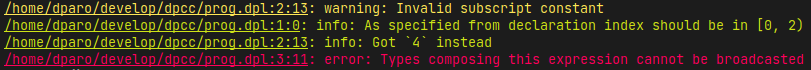
\includegraphics[width=\linewidth]{imgs/log.png}
        \caption{\texttt{dpcc} custom logging showoff}
    \end{figure}


\subsubsection{Typescript code generation}

Without going too much deeper on the details, some part of the C source code composing the compiler is in fact
generated using a \textbf{Typescript} program. Having now more knowledge about how the compiler source code
turned out to be at the end, the decision of generating some part of the compiler turned
out to be mostly \textbf{overkill}; especially considering the small size of the project. But anyway this
trick is something that I wanted to try and see if it works. I didn't gain much using this code generation
trick but I still think that theoretically speaking it could help in managing
the source code of the compiler as it increases in scale.

Without spending too much time on this section, the \textbf{Typescript} program is used to do two things:

\begin{itemize}
    \item To generate the code for the type deduction and type checking of the each expression operator. It takes
        some \textbf{meta-representations} of what each expression accept as input types and which output type it produces.
        Given these \textbf{meta-representations} it generates a C function called \texttt{typecheck\_expr\_and\_operators} and some other utilities in a separate C file which is then compiled in the final executable.
        An example of such \textbf{meta-representation} is:
        \begin{lstlisting}[language=JS]
const MATH_EXPR = new Expr (
    [
        "ExprAdd", "ExprSub", "ExprMul", "ExprDiv", "ExprPow",
        "ExprInc", "ExprDec", "ExprPos", "ExprNeg",
    ],
    [
        new ExprTypeRule("int", ["int", "int"]),
        new ExprTypeRule("float", ["float", "int"]),
        new ExprTypeRule("float", ["int", "float"]),
        new ExprTypeRule("float", ["float", "float"]),

        new ExprTypeRule("int", ["int"]),
        new ExprTypeRule("float", ["float"]),
    ]
);
        \end{lstlisting}

    which rougly says that operators such as \texttt{+, -, *, /, **, ++, \dots} can either take integers or floats as inputs,
    and depending on which input types are provided, it either produces an \texttt{int} or \texttt{float} type as output.

    \item To embed the required preamble and postamble C code inside the \texttt{dpcc} executable. The preamble and
        postamble code that are outputted when calling \texttt{`./dpcc c <input>'} are in fact written
        into two separate files. The typescript program reads these two files and generate two header files
        containing two \texttt{uint8\_t[]} arrays that each encode the content of each respective file. Then
        these two generated \texttt{uint8\_t} arrays are then embedded in the final executable.
\end{itemize}


\subsubsection{Custom allocator wrapper}

In order to track allocations inside the compiler a simple custom allocator is implemented.
In practice this allocator just wraps the standard C allocator (\texttt{malloc}) and stores each allocation
in a list. The reason for this is that one can simply allocate memory as he/she likes without worrying about freeing
such memory. If the structure of the program is correctly thought out, one can simply define good synchronization
points where it is safe to clear the entire allocator. Thus all allocations made up to this point
can all be freed at once. One can also use multiple allocators to model different lifetime semantics for objects
that must live longer or shorter.

The custom allocator lives in \texttt{src/utils.c} and the notable functions are:\texttt{dallnew, dallrsz, dalldel, dallclr, dallarr, \dots}.


\subsection{Testing framework}

The \texttt{dpcc} compiler has unit testing framework setup to make sure that the compiler works as expected.
The library \urlref{https://github.com/ThrowTheSwitch/Unity}{Unity} is a standalone unit framework written C. The
\texttt{dpcc} uses this library to test some utilities freestanding functions in isolation.

Most of the testing horsepower is provided by a \urlref{https://www.python.org/}{Python} script: \texttt{test/compile\_test.py}.
This script reads 2 files: \texttt{test/valid.dpl, test/invalid.dpl} which list respectively some valid and invalid dpl programs.
Each program is separated by a long sequence of characters \texttt{`//'}. The python script extract each program
separately, for each program it extract some metadata from the comments which list the expected output of the program.
The python script then proceeds to call the compiler on that small program and verifies that either the program
produces the expected output, or in the case of invalid programs it rejects it without crashing.


This is an example taken directly from \texttt{test/valid.dpl}:

\begin{lstlisting}[language=DPL]
//@ Boolean var decls
//@ t = 1
//@ 0

print("\n\nBoolean var decls\n");
{
    let t = true;
    print(t);
    print(false);
}

///////////////////////////////////////////////////////////////////////////////

//@ Integer array type deduction
//@ a = [ 10, 20, 30, 40, 50 ]
//@ a = [ 10, 20, 30, 40, 100 ]

print("\n\nInteger array type deduction\n");
{
    let a = [ 10, 20, 30, 40, 50 ];
    print(a);
    a[4] = 100;
    print(a);
}
///////////////////////////////////////////////////////////////////////////////
\end{lstlisting}

Notice the program separator and how the metadata is instead listed in a comment beginning with \texttt{//@}.

Here's instead some examples from \texttt{test/invalid.dpl}:

\begin{lstlisting}[language=DPL]
// Integer is too large
{
    let a = 10000000000000000000;
    print(a);
}
///////////////////////////////////////////////////////////////////////////////

// Arrays with no RHS must be sized
{
    let b: int[];
}
///////////////////////////////////////////////////////////////////////////////

// Arrays must have reasoanble size
{
    let a: int[-1];
}
///////////////////////////////////////////////////////////////////////////////

// Array with RHS must have correct size
{
    let a: int[3] = [ 2, 3 ];
}
///////////////////////////////////////////////////////////////////////////////
\end{lstlisting}


\clearpage

\section{Performance results}

\urlref{https://www.valgrind.org/}{Valgrind} is a very useful tool for C development. It is primarily used for
memory debugging (memory corruptions, invalid writes acccess, \dots), finding memory leaks, and for
profiling (timing, cache hit rate, branch prediction, \dots). Some memory bugs were totally eliminated
inside the compiler thanks to this tool. Thanks to \textbf{valgrind}, also, some performance analysis abot the
total running time of the compilar were analysed (\texttt{valgrind --tool=callgrind --dump-instr=yes --simulate-cache=yes --collect-jumps=yes -- \dots}).

As it turned out from the analysis currently the compiler has un-satisfactory performance. The performance analysis
highlighted the current custom allocator implementation is the \textbf{bottleneck} of the compiler. Most
of the running time of the compiler is \textbf{wasted} on performing linear searches for allocation resizes.

As one can see from the below images, the \texttt{dallrsz} function, and in particular the linear scanning of the allocation
consitutes more than \textbf{99\%} of the total running time of the executable.

This problem is something that should totally be addressed before shipping the \texttt{dpcc} compiler to a final user.

Also I wanted to take some snapshots about the running time of the compilar as a function of the  source code input
size. Unfortunately since the current implementation of the allocator is \textbf{slow}, such snapshots
wouldn't provide much information about how fast the compilation process is.

\begin{figure}[H]
    \centering
    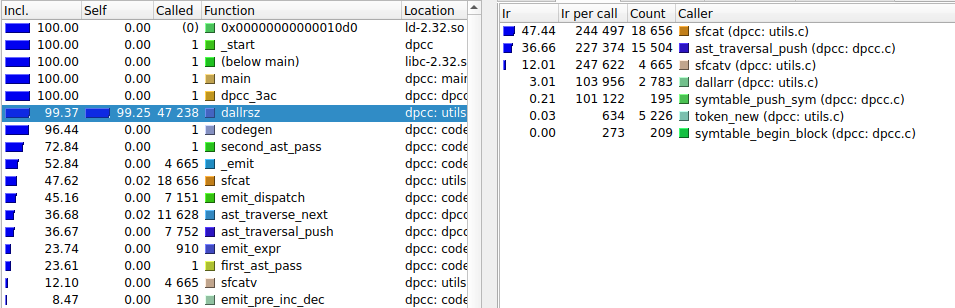
\includegraphics[width=\linewidth]{imgs/dallrsz_performance_issue.png}
    \caption{Performance issue in \texttt{dallrsz} utility function.}
\end{figure}


\begin{figure}[H]
    \centering
    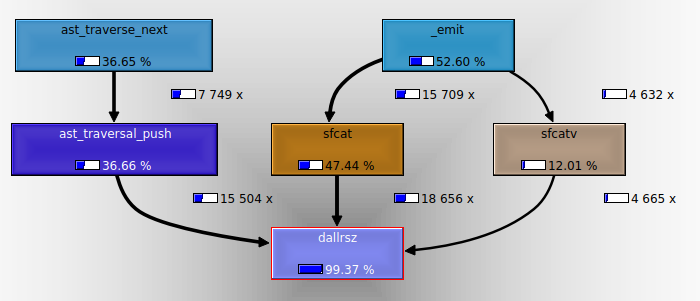
\includegraphics[scale=0.85]{imgs/dallrsz_callgraph.png}
    \caption{Performance issue same as previous image but in a graph form.}
\end{figure}


\begin{figure}[H]
    \centering
    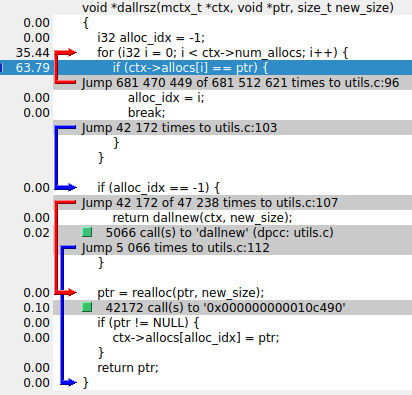
\includegraphics{imgs/dallrsz_code_usage.png}
    \caption{The linear search allocation scanning. The loop is taken tramendous amount of time for basically no useful reason.}
\end{figure}


\clearpage

\section{Conclusions}

The \textbf{DPL} language and the \textbf{dpcc} compiler are far from being useful and/or complete.
They were implemented as part of a course in Compilers, so it is mostly a proof of concept. But still
this proof of concept apply some modern features that languages
like C lacks in its standard (type deduction, proper precedence table, proper fixed sized integers).

That being said, I still find that both this implementation and project report provide some concepts that are still applicable in a proper language \& compiler implementation.
The language mostly lacks proper features to be useful as an everyday productive language (procedure calls are a must).
Also the compiler lacks a  real-world efficient code generation backend. Unfortunately nowadays, due to the complexity
of modern CPU architectures, writing a compiler backend is not an easy task. In fact most modern languages
nowadays rely on external backends such as \textbf{LLVM}\footnote{\urlref{https://llvm.org/}{LLVM Website}} to deal with the actual machine code output.

It would be cool to extend this language and bring it further. It would probably need some code refactoring/cleanup first,
but the unit testing framework should help in that. Some cool concepts that could be investigated further are:

\begin{itemize}
\item \textbf{FUNCTIONS !!!}
\item More basic types
\item Custom definable types: struct, unions, possibly classes
\item Namespaces to avoid the dependency hell that C has
\item Proper metaprogramming system which is language and type aware (avoid C preprocessors macros)
\item Proper module system
\item Infrastracture: build system, package manager, tooling, and more \dots
\item \dots
\end{itemize}

\clearpage
\section{Appendix A: Example Program: Iterative Merge Sort}
\label{appendix_a}

\subsection{Input DPL source}

\begin{lstlisting}[language=DPL]
let len = 32;
let array = [
    15, 59, 61, 75, 12, 71,  5, 35, 44,
    6, 98, 17, 81, 56, 53, 31, 20, 11,
    45, 80,  8, 34, 71, 83, 64, 28,  3,
    88, 50, 48, 80,  5
];


print("Un-sorted array\n");
print(array);

{
    for (let cs = 1; cs < len; cs = 2 * cs) {
        for (let l = 0; l < len - 1; l = l + 2 * cs) {
            let m = len - 1;
            if ((l + cs - 1) < len - 1) {
                m = l + cs - 1;
            }
            let r = len - 1;
            if ((l + 2 * cs - 1) < len - 1) {
                r = l + 2 * cs - 1;
            }


            let n1 = m - l + 1;
            let n2 = r - m;

            let L: int[1024];
            let R: int[1024];

            // Copy to temp arrays
            for (let i = 0; i < n1; i++) {
                L[i] = array[l + i];
            }
            for (let i = 0; i < n2; i++) {
                R[i] = array[m + 1 + i];
            }


            let i = 0;
            let j = 0;
            let k = l;
            while (i < n1 && j < n2) {
                if (!(L[i] > R[j])) {
                    array[k++] = L[i++];
                } else {
                    array[k++] = R[j++];
                }
            }

            while (i < n1) {
                array[k++] = L[i++];
            }
            while (j < n2) {
                array[k++] = R[j++];
            }
        }
    }
}

print("\nSorted array\n");
print(array);
\end{lstlisting}

\clearpage

\subsection{Obtained output}
\begin{lstlisting}
Un-sorted array
array = [ 15, 59, 61, 75, 12, 71, 5, 35, 44, 6, 98, 17, 81, 56, 53, 31, 20, 11, 45, 80, 8, 34, 71, 83, 64, 28, 3, 88, 50, 48, 80, 5 ]

Sorted array
array = [ 3, 5, 5, 6, 8, 11, 12, 15, 17, 20, 28, 31, 34, 35, 44, 45, 48, 50, 53, 56, 59, 61, 64, 71, 71, 75, 80, 80, 81, 83, 88, 98 ]
\end{lstlisting}



\subsection{Emitted 3AC code}


\begin{lstlisting}[language=C]

// Special variable used to implemenent INC (x++) and dec (x--)
// It is used to temporary hold the result of the INC/DEC in order to perform the side effect
int32_t _vspcIncDec;
// Special variable used for the negation of control statements (if, for, ...)
// As an example the for loop needs to negate the user provided condition
bool    _vspcNeg;

// 3AC Var decls
int32_t _vi0 = 0;
int32_t _vi1 = 0;
int32_t _vi2 = 0;
int32_t _vi3 = 0;
int32_t _vi4 = 0;
int32_t _vi5 = 0;
int32_t _vi6 = 0;
int32_t _vi7 = 0;
int32_t _vi8 = 0;
int32_t _vi9 = 0;
int32_t _vi10 = 0;
int32_t _vi11 = 0;
int32_t _vi12 = 0;
int32_t _vi13 = 0;
int32_t _vi14 = 0;
int32_t _vi15 = 0;
int32_t _vi16 = 0;
int32_t _vi17 = 0;
int32_t _vi18 = 0;
int32_t _vi19 = 0;
int32_t _vi20 = 0;
int32_t _vi21 = 0;
int32_t _vi22 = 0;
int32_t _vi23 = 0;
int32_t _vi24 = 0;
int32_t _vi25 = 0;
int32_t _vi26 = 0;
int32_t _vi27 = 0;
int32_t _vi28 = 0;
int32_t _vi29 = 0;
int32_t _vi30 = 0;
int32_t _vi31 = 0;
int32_t _vi32 = 0;
int32_t _vi33 = 0;
int32_t _vi34 = 0;
int32_t _vi35 = 0;
int32_t _vi36 = 0;
int32_t _vi37 = 0;
int32_t _vi38 = 0;
int32_t _vi39 = 0;
int32_t _vi40 = 0;
int32_t _vi41 = 0;
int32_t _vi42 = 0;
int32_t _vi43 = 0;
int32_t _vi44 = 0;
int32_t _vi45 = 0;
int32_t _vi46 = 0;
int32_t _vi47 = 0;
int32_t _vi48 = 0;
int32_t _vi49 = 0;
int32_t _vi50 = 0;
int32_t _vi51 = 0;
int32_t _vi52 = 0;
int32_t _vi53 = 0;
int32_t _vi54 = 0;
int32_t _vi55 = 0;
int32_t _vi56 = 0;
int32_t _vi57 = 0;
bool    _vb0 = false;
bool    _vb1 = false;
bool    _vb2 = false;
bool    _vb3 = false;
bool    _vb4 = false;
bool    _vb5 = false;
bool    _vb6 = false;
bool    _vb7 = false;
bool    _vb8 = false;
bool    _vb9 = false;
bool    _vb10 = false;
bool    _vb11 = false;
bool    _vb12 = false;

_scope_begin();
    _var_decl("len", _kI32, 1);
    _var_init("len", _kI32, 1, (int32_t[]) {32});
    _var_decl("array", _kI32, 32);
    _var_init("array", _kI32, 32, (int32_t[]) {15, 59, 61, 75, 12, 71, 5, 35, 44, 6, 98, 17, 81, 56, 53, 31, 20, 11, 45, 80, 8, 34, 71, 83, 64, 28, 3, 88, 50, 48, 80, 5});
    printf("%s", "Un-sorted array\n");
    print_sym("array");
    _scope_begin();
        _scope_begin();
            _var_decl("cs", _kI32, 1);
            _var_init("cs", _kI32, 1, (int32_t[]) {1});
            _lbl18:
            _vb0 = _var_get_kI32("cs", 0) < _var_get_kI32("len", 0);
            _vspcNeg = !_vb0;
            if (_vspcNeg) goto _lbl19;
            _scope_begin();
                _scope_begin();
                    _var_decl("l", _kI32, 1);
                    _var_init("l", _kI32, 1, (int32_t[]) {0});
                    _lbl16:
                    _vi0 = _var_get_kI32("len", 0) - 1;
                    _vb1 = _var_get_kI32("l", 0) < _vi0;
                    _vspcNeg = !_vb1;
                    if (_vspcNeg) goto _lbl17;
                    _scope_begin();
                        _var_decl("m", _kI32, 1);
                        _vi1 = _var_get_kI32("len", 0) - 1;
                        _var_init("m", _kI32, 1, (int32_t[]) {_vi1});
                        _vi2 = _var_get_kI32("l", 0) + _var_get_kI32("cs", 0);
                        _vi3 = _vi2 - 1;
                        _vi4 = _var_get_kI32("len", 0) - 1;
                        _vb2 = _vi3 < _vi4;
                        _vspcNeg = !_vb2;
                        if (_vspcNeg) goto _lbl1;
                        _scope_begin();
                            _vi5 = _var_get_kI32("l", 0) + _var_get_kI32("cs", 0);
                            _vi6 = _vi5 - 1;
                            _vi7 = _var_set_kI32("m", 0, _vi6);
                        _scope_end();
                        _lbl1:
                        _var_decl("r", _kI32, 1);
                        _vi8 = _var_get_kI32("len", 0) - 1;
                        _var_init("r", _kI32, 1, (int32_t[]) {_vi8});
                        _vi9 = 2 * _var_get_kI32("cs", 0);
                        _vi10 = _var_get_kI32("l", 0) + _vi9;
                        _vi11 = _vi10 - 1;
                        _vi12 = _var_get_kI32("len", 0) - 1;
                        _vb3 = _vi11 < _vi12;
                        _vspcNeg = !_vb3;
                        if (_vspcNeg) goto _lbl3;
                        _scope_begin();
                            _vi13 = 2 * _var_get_kI32("cs", 0);
                            _vi14 = _var_get_kI32("l", 0) + _vi13;
                            _vi15 = _vi14 - 1;
                            _vi16 = _var_set_kI32("r", 0, _vi15);
                        _scope_end();
                        _lbl3:
                        _var_decl("n1", _kI32, 1);
                        _vi17 = _var_get_kI32("m", 0) - _var_get_kI32("l", 0);
                        _vi18 = _vi17 + 1;
                        _var_init("n1", _kI32, 1, (int32_t[]) {_vi18});
                        _var_decl("n2", _kI32, 1);
                        _vi19 = _var_get_kI32("r", 0) - _var_get_kI32("m", 0);
                        _var_init("n2", _kI32, 1, (int32_t[]) {_vi19});
                        _var_decl("L", _kI32, 1024);
                        _var_decl("R", _kI32, 1024);
                        _scope_begin();
                            _var_decl("i", _kI32, 1);
                            _var_init("i", _kI32, 1, (int32_t[]) {0});
                            _lbl4:
                            _vb4 = _var_get_kI32("i", 0) < _var_get_kI32("n1", 0);
                            _vspcNeg = !_vb4;
                            if (_vspcNeg) goto _lbl5;
                            _scope_begin();
                                _vi20 = _var_get_kI32("L", _var_get_kI32("i", 0));
                                _vi21 = _var_get_kI32("l", 0) + _var_get_kI32("i", 0);
                                _vi22 = _var_get_kI32("array", _vi21);
                                _vi23 = _var_set_kI32("L", _var_get_kI32("i", 0), _vi22);
                            _scope_end();
                            _vi24 = _var_get_kI32("i", 0);
                            _vspcIncDec = _var_get_kI32("i", 0) + 1;
                            _var_set_kI32("i", 0, _vspcIncDec);
                            goto _lbl4;
                            _lbl5:
                        _scope_end();
                        _scope_begin();
                            _var_decl("i", _kI32, 1);
                            _var_init("i", _kI32, 1, (int32_t[]) {0});
                            _lbl6:
                            _vb5 = _var_get_kI32("i", 0) < _var_get_kI32("n2", 0);
                            _vspcNeg = !_vb5;
                            if (_vspcNeg) goto _lbl7;
                            _scope_begin();
                                _vi25 = _var_get_kI32("R", _var_get_kI32("i", 0));
                                _vi26 = _var_get_kI32("m", 0) + 1;
                                _vi27 = _vi26 + _var_get_kI32("i", 0);
                                _vi28 = _var_get_kI32("array", _vi27);
                                _vi29 = _var_set_kI32("R", _var_get_kI32("i", 0), _vi28);
                            _scope_end();
                            _vi30 = _var_get_kI32("i", 0);
                            _vspcIncDec = _var_get_kI32("i", 0) + 1;
                            _var_set_kI32("i", 0, _vspcIncDec);
                            goto _lbl6;
                            _lbl7:
                        _scope_end();
                        _var_decl("i", _kI32, 1);
                        _var_init("i", _kI32, 1, (int32_t[]) {0});
                        _var_decl("j", _kI32, 1);
                        _var_init("j", _kI32, 1, (int32_t[]) {0});
                        _var_decl("k", _kI32, 1);
                        _var_init("k", _kI32, 1, (int32_t[]) {_var_get_kI32("l", 0)});
                        _lbl10:
                        _vb6 = _var_get_kI32("i", 0) < _var_get_kI32("n1", 0);
                        _vb7 = _var_get_kI32("j", 0) < _var_get_kI32("n2", 0);
                        _vb8 = _vb6 && _vb7;
                        _vspcNeg = !_vb8;
                        if (_vspcNeg) goto _lbl11;
                        _scope_begin();
                            _vi31 = _var_get_kI32("L", _var_get_kI32("i", 0));
                            _vi32 = _var_get_kI32("R", _var_get_kI32("j", 0));
                            _vb9 = _vi31 > _vi32;
                            _vb10 = ! _vb9;
                            _vspcNeg = !_vb10;
                            if (_vspcNeg) goto _lbl8;
                            _scope_begin();
                                _vi33 = _var_get_kI32("k", 0);
                                _vspcIncDec = _var_get_kI32("k", 0) + 1;
                                _var_set_kI32("k", 0, _vspcIncDec);
                                _vi34 = _var_get_kI32("array", _vi33);
                                _vi35 = _var_get_kI32("i", 0);
                                _vspcIncDec = _var_get_kI32("i", 0) + 1;
                                _var_set_kI32("i", 0, _vspcIncDec);
                                _vi36 = _var_get_kI32("L", _vi35);
                                _vi37 = _var_set_kI32("array", _vi33, _vi36);
                            _scope_end();
                            goto _lbl9;
                            _lbl8:
                            _scope_begin();
                                _vi38 = _var_get_kI32("k", 0);
                                _vspcIncDec = _var_get_kI32("k", 0) + 1;
                                _var_set_kI32("k", 0, _vspcIncDec);
                                _vi39 = _var_get_kI32("array", _vi38);
                                _vi40 = _var_get_kI32("j", 0);
                                _vspcIncDec = _var_get_kI32("j", 0) + 1;
                                _var_set_kI32("j", 0, _vspcIncDec);
                                _vi41 = _var_get_kI32("R", _vi40);
                                _vi42 = _var_set_kI32("array", _vi38, _vi41);
                            _scope_end();
                            _lbl9:
                        _scope_end();
                        goto _lbl10;
                        _lbl11:
                        _lbl12:
                        _vb11 = _var_get_kI32("i", 0) < _var_get_kI32("n1", 0);
                        _vspcNeg = !_vb11;
                        if (_vspcNeg) goto _lbl13;
                        _scope_begin();
                            _vi43 = _var_get_kI32("k", 0);
                            _vspcIncDec = _var_get_kI32("k", 0) + 1;
                            _var_set_kI32("k", 0, _vspcIncDec);
                            _vi44 = _var_get_kI32("array", _vi43);
                            _vi45 = _var_get_kI32("i", 0);
                            _vspcIncDec = _var_get_kI32("i", 0) + 1;
                            _var_set_kI32("i", 0, _vspcIncDec);
                            _vi46 = _var_get_kI32("L", _vi45);
                            _vi47 = _var_set_kI32("array", _vi43, _vi46);
                        _scope_end();
                        goto _lbl12;
                        _lbl13:
                        _lbl14:
                        _vb12 = _var_get_kI32("j", 0) < _var_get_kI32("n2", 0);
                        _vspcNeg = !_vb12;
                        if (_vspcNeg) goto _lbl15;
                        _scope_begin();
                            _vi48 = _var_get_kI32("k", 0);
                            _vspcIncDec = _var_get_kI32("k", 0) + 1;
                            _var_set_kI32("k", 0, _vspcIncDec);
                            _vi49 = _var_get_kI32("array", _vi48);
                            _vi50 = _var_get_kI32("j", 0);
                            _vspcIncDec = _var_get_kI32("j", 0) + 1;
                            _var_set_kI32("j", 0, _vspcIncDec);
                            _vi51 = _var_get_kI32("R", _vi50);
                            _vi52 = _var_set_kI32("array", _vi48, _vi51);
                        _scope_end();
                        goto _lbl14;
                        _lbl15:
                    _scope_end();
                    _vi53 = 2 * _var_get_kI32("cs", 0);
                    _vi54 = _var_get_kI32("l", 0) + _vi53;
                    _vi55 = _var_set_kI32("l", 0, _vi54);
                    goto _lbl16;
                    _lbl17:
                _scope_end();
            _scope_end();
            _vi56 = 2 * _var_get_kI32("cs", 0);
            _vi57 = _var_set_kI32("cs", 0, _vi56);
            goto _lbl18;
            _lbl19:
        _scope_end();
    _scope_end();
    printf("%s", "\nSorted array\n");
    print_sym("array");
_scope_end();
\end{lstlisting}

% \section{Appendix: test cases} % Optional
%
% ...

% \section{Appendix: Extensions} % Optional
%
% ...

\end{document}
